\section{Policy-compliant Resiliency}
Datacenter networks are highly prone to failures, 
and it is crucial to ensure certain guarantees during such failure
situations. For example, if the operator want to guarantee
reachability amongst endpoints, the controller has to find a active
path in the network to re-establish reachability. However, if the new
paths must still satisfy tenant SLAs like isolation, this may require 
changing paths of other classes which were unaffected by the failure event,
and in the worst case, can incur an exponential complexity.
While \name provides a systematic and correct approach
to enforcing policies, the implications of using SMT solvers is that
it is very difficult to be able to synthesize configuration repairs to
network failures \emph{reactively} in a bounded amount of time. 
Instead, we propose a \emph{proactive} approach 
of support for \emph{policy-compliant resiliency} to tackle network failures
by synthesizing backup paths which satisfy the input policies, such that the SDN controller 
can choose an alternate path in the scenario of a link/switch failure with no
policy violations.

\begin{mydef}
	$t-resilience$ synthesis for a packet class is defined as the
	synthesis of paths such that in the event of upto arbitary
	$t$ link failures, there exists a synthesized path for the packet class which
	satisfies the input policies. 
\end{mydef}

We leverage link-isolation where paths do not share a link in both directions 
(different from traffic isolation)
 as a means to provide $t-resilience$ for a packet class. For a 
packet class $pc$, we create $t$ replicas of the reachability policy with waypoints (if specified)
to create a total of $t+1$ packet classes. For resilience, we add link-isolation policies among each
of these packet classes so that we get $t+1$ edge disjoint paths from source to destination
(passing through waypoints, if specified). Thus, in the event of arbitary $t$ link failures, the 
controller can choose one of the $t+1$ paths unaffected by the link failures as the primary
path for the packet class. 

This transformation is sound and complete. The proof sketch for soundness
 is as follows: suppose a $t$ link failure
disables all $t+1$ paths, which would mean there is one link which disables atleast two paths
of the packet class. This is a contradiction, as the paths are edge-disjoint from each other, and one
link failure can affect one path at maximum. The proof sketch for completeness is as follows:
suppose there are $t+1$ resilient paths such that they are not all edge-disjoint, i.e atleast two
paths share an edge. Choose this edge, and $t-1$ edges from remaining $t-1$ paths, and
thus, we have a $t$ link failure scenario which affects all paths. Therefore, the $t+1$ resilient
paths have to be edge-disjoint.
\begin{figure}
	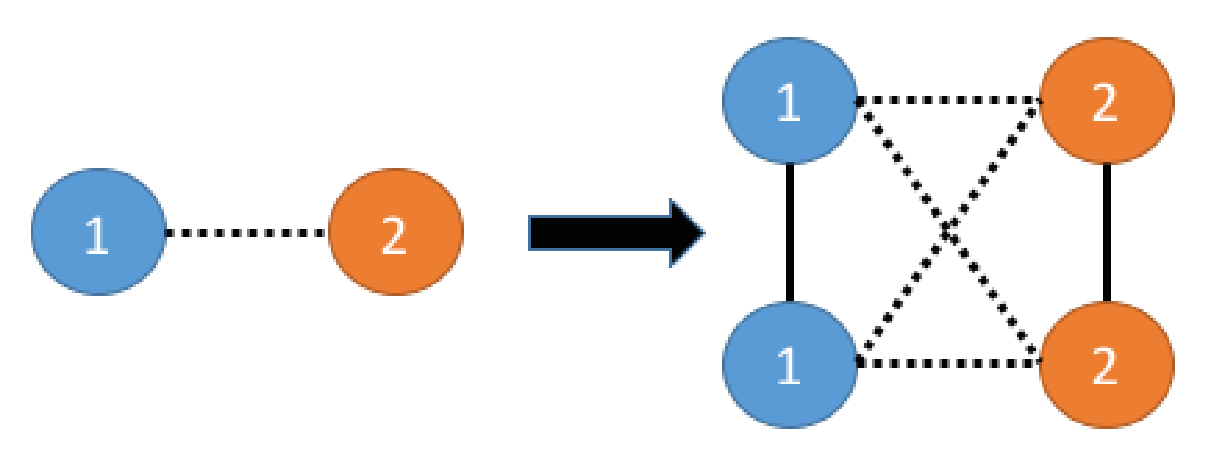
\includegraphics[width=0.8\columnwidth,center]{figures/resilience-transform.eps}
	\compactcaption{Resilience Transformation for $pc_1 || \ pc_2$ for providing $1-resilience$. The dotted lines represent traffic isolation policies, while the solid lines represent link isolation.}
	\label{fig:restransform}
\end{figure}
To extend this transformation for isolation policies, consider two packet class $pc_1 ||\ pc_2$. 
To provide $t-resilience$ to only $pc_1$, we apply the transformation to $pc_1$ as described
earlier, and add isolation policies for all the $t+1$ packet classes of $pc_1$ to $pc_2$,
thus ensuring that all paths of $pc_1$ are isolated to $pc_2$ under any arbitary $t$ link 
failure scenario. For $t-resilience$ synthesis for both $pc_1$ and $pc_2$, the transformation
is shown in \Cref{fig:restransform}.

This transformation is sound, as all paths of $pc_1$ are isolated to all paths of $pc_2$,
therefore, irrespective of whichever pair of paths are chosen for $pc_1$ and $pc_2$,
they will satisfy $pc_1 || \ pc_2$.
\kausik{Dont know about completeness!}
 However, this transformation is not complete (refer to 
figure showing counter-ex). 

We presented a sound transformation of policies to provide $t-resilience$ in
the case of reachability, waypoint and isolation policies. However, for global policies like 
traffic engineering, $t-resilience$ synthesis is complicated as the $t$ backup paths 
cannot be considered simply as different packet classes (they do not exist at the same time
in the network),
and thus cannot be considered in the optimization objective. Therefore, we require a 
temporal notion of the objective (like average link utilization) across link failures. Synthesis of resilient paths
satisfying traffic engineering objectives is one of the future directions of research.